\chapter{Literature Review}

This chapter outlines the existing systems being used to predict the safety of drinking water sources in Bangladesh and other regions where applicable, the tooling and techniques required to implement and evaluate new prediction models and touches on the considerations and limitations of these models with regard to the black box problem. 

\section{Existing Work}
\label{ew}

\subsection{iArsenic}

The existing iArsenic models are expert system models. This type of model follows rules defined by an expert in the field, this can be thought of as a flow chart. This approach has the benefit of the output of the model being explainable and justifiable; a white box model. 

Expert systems can be limited compared to machine learning-based models as the decision boundaries made by an expert system are defined by an expert, whereas machine learning algorithms will statistically identify decision boundaries.

In total there are 5 iArsenic models, each has been developed sequentially, improving on the one before. Initially written in R, 3 of the iArsenic models, model3, model4 and model5, have been converted to NodeJS / JavaScript and uploaded to GitHub.

The iArsenic models are documented at this link: \url{https://github.com/portsoc/iArsenic/tree/master/preprocessing}

\subsection{Predicting Arsenic Concentrations with Surface Parameters}

\cite{Winkel2008} page 536 used latitude, longitude and surface parameters from the Food and Agriculture Organization of the United Nations to predict arsenic concentration in groundwater. This was done by calculating the correlation coefficient between these surface parameters and arsenic concentrations for use as global parameters in a classification model. This model achieved a true positive and true negative rate of 65\% over multiple countries in Southeast Asia.

\subsection{Satellite Mapping of Flooding Patterns}

\cite{Connolly2022} page 928 uses high-resolution satellite data combined with surface parameters to predict groundwater arsenic concentrations within an area of 30m using a random forest model. The results in this article are not comprehensive, though a figure for a sensitivity rate of 95\% for wells with arsenic concentrations of over 10µg/l is provided.

The compromise for this high sensitivity level appears to be that the dataset covers a smaller area than the iArsenic dataset, which covers the majority of Bangladesh or \cite{Winkel2008}'s dataset which covers several countries in Southeast Asia.

\textbf{Conclusion}

While \cite{Connolly2022}'s model achieving a sensitivity rate of 95\% is the highest for any model found in this literature review, this does not provide a comprehensive performance evaluation for the model. A model which always predicts true will have a sensitivity of 1.

\cite{Winkel2008}'s model provides a more robust evaluation by providing a receiver operator curve.

It is not possible to generate a receiver operator curve for the iArsenic models. This is because the models do not provide a feature to change the classification threshold. It is possible to generate the f1 score, sensitivity and specificity. This will factor in the true positive rate and true negative rate. See these terms defined at \ref{EM} on page \pageref{EM}.

\section{The Black Box Problem}

\cite{Fleming2021} states that acceptance of machine learning-based approaches have faced resistance in earth \& environmental sciences due to the inability to explain how machine learning models are working and the lack of understanding of artificial intelligence in the earth \& environmental field. While this is partially true in terms of the black box problem there is are examples of machine learning being used to analyze groundwater quality. A more difficult question to answer is whether these models are less applicable in real life compared to human-designed models, as is asserted by \cite{Guidotti2018}.

In machine learning, the black box problem is based on the inability to explain how a model produces an output for a given input.

\cite{Castelvecchi2016} illustrates this issue with the following, imagine a black box machine learning model was created with a set of images of mammograms including labels indicating whether the person in the scan went on to develop breast cancer. It could happen that this model outperforms human medical professionals in predicting whether someone would go on to develop breast cancer.

One could argue that the benefit of this model would be that it could identify when women should have a preventative mastectomy. However, critics assert that critical decisions cannot be made without justification and that one cannot justify a decision that cannot be explained (\cite{Loyola-Gonzalez2019}). The human doctor's opinion will always be explainable, by the doctor themselves.

Not all machine learning base models are considered to be black box systems. Decision tree models for example are powerful machine learning tools which produce models considered white box systems meaning you can analyse them to determine how they're working \parencite{Caruana2006}. Decision tree models can be contrasted with neural network style models which are almost always considered black box models.

Because determining whether a drinking water source is safe does factor into critical decision-making, it is important to explore the black box problem. The purpose of this project, however, is to compare the performance of a predictive model developed with machine learning to existing expert system models. Therefore whether a model is black or white box will not be a critical factor in model selection.

\section{Tool Selection}

\subsection{Model Implementation}

Preliminary investigations into machine learning, including speaking to local experts at the University of Portsmouth, identified three potential systems for designing and implementing machine learning frameworks, scikit-learn, WEKA and TensorFlow.

\textbf{scikit-learn}

Scikit-learn provides a well defined Python interface for a wide range of well defined machine learning models and techniques. This makes scikit-learn good for implementing existing model architecture but limits the development of new architectures. This makes scikit-learn less suitable for custom architectures and deep learning than tools such as TensorFlow. 

Its Python interface does mean however that it does not limit the possibilities of preprocessing or post-processing the input and output of a model (\cite{scikit-learn2023}).

\textbf{TensorFlow}

TensorFlow contrasts with scikit-learn by allowing full access to the model architecture. This makes it suitable for both deep learning and supervised learning. TensorFlow can also follow a distributed architecture, allowing it to scale to larger datasets. This versatility however greatly increases the complexity of the tool in comparison to WEKA or scikit-learn (\cite{Google2023}).

TensorFlow provides GPU support, which could be used to decrease the time taken when testing and training, allowing less optimization to be applied to models.

\textbf{WEKA}

Of the three tools for model implementation considered, WEKA is the most simple to use, providing a graphical user interface. While this simplicity means WEKA is very easy to use, it is also limited in its versatility, providing a limited API, making it difficult to integrate with the iArsenic models and fewer model types and configuration options compared to scikit-learn or TensorFlow (\cite{Waikato2023}).

\textbf{Conclusion}

Scikit-learn has been chosen to develop and run the models because of its standardised Python based model interface. WEKA was not deemed suitable because it provides no easy way to integrate with Python or NodeJS. TensorFlow would be a suitable choice but is less appropriate than scikit-learn due to the complexity it introduces.

\subsection{Python Dependency Management}

This section will outline and compare the potential choices for dependency management.

Good dependency management allows a Python project to be added to a different machine and for that project's dependencies to be installed without clashing with the existing Python dependencies of that system. Without this, the code can become tied to the developer's system-wide Python installation and prevent other Python projects from being unable to run, where they require different versions of the same package as another Python project on the system.

\textbf{Conda}

Conda is a high-level environment and package dependency manager which works with Python and other languages. The appeal of Conda is the simplicity of the user experience. Conda manages every aspect of environment and dependency management. This, however, comes at the cost of the complexity of the tool itself. Portability and collaboration is a concern with Conda, as to run it on a virtual machine or another developer's machine, this machine will also need Conda to be installed, which may clash with existing dependency management solutions (\cite{Conda2023}).

\textbf{Virtualenv}

With virtualenv, isolated Python environments can be created and stored in a directory of the project (\cite{virtualenv2023}).

Used in conjunction with the Python package manager, pip, dependencies can be installed to this isolated environment and their version tracked using the pip freeze command. The output of the pip freeze command is conventionally stored in a file named requirements.txt. The requirements.txt file can then be included with the source code and used to install the specific dependencies required for a project.

\textbf{pipenv}

The aim of pipenv is to integrate virtualenv and pip, making it a higher-level alternative to using virtualenv with pip. Practically, the benefit of pipenv is the use of a package.lock file, which allows dependencies to be locked to a specific version, providing a security benefit. This feature however does add complexity and maintainability requirements (\cite{Reitz2023}).

\textbf{Conclusion}

Ultimately virtualenv was chosen for this project due to it being the most simple and lightweight solution, reducing the number of potential failure points when porting to other systems or coming back to this project in the future.

\section{Model Type}
\label{mt}

The initial steps in model selection are rudimentary. Machine learning algorithms can be categorised as, supervised learning, semisupervised learning, unsupervised learning and reinforcement learning. Because our data set consists of structured and labelled data the appropriate choice is supervised learning, see \cite{Aurélien2017} page 24.

Predictions by the existing iArsenic models classify data points as safe, polluted or highlyPolluted. Models produced in this project therefore must produce a comparable output. Predictions from a regression model will not be as comparable to predictions from an iArsenic model as a regression model will output a continuous value. While this would produce valid predictions, it would not be applicable in this project because this estimate will have to be converted to a classification. Therefore the models considered for this project are classification based.

% TODO expand on how these models work

Rich Caruana and Alexandru Niculescu-Mizil provide a comparison of a number of supervised learning algorithms on a range of data sets and performance measures (\cite{Caruana2006}). Based on Caruana's paper and \cite{Aurélien2017} chapter 3, the following model types have been shortlisted for their good performance across a diverse range of dataset types:
\begin{itemize}
    \item k-nearest neighbors classifier
    \item random forest classifier
    \item multilayer perceptron feed forward neural network classifier
\end{itemize}

\subsection{Validating Models \& Minimizing Dataset Bias}
\label{eval}

Bias is always a factor in datasets, some types of bias cannot be measured or controlled, such as sampling bias focusing on collecting data points in and around a city's capital with less focus on rural regions. This may be the case in the dataset used in this project, but further scrutinizing bias is outside the scope of this project. 

The impact of ordering and sampling bias can be minimized however, this section will explore the ways this can be done.

\textbf{Hold Out Validation}

In hold-out validation, the dataset is split into two, a test set and a train set. The train set is used to train a model, then the model is presented with new data to make predictions for. 

This proves the model can generalize to new data, validating its performance. This method is susceptible to ordering and sample bias, however, if for example the dataset is ordered alphabetically.

\textbf{K-folds Cross Validation}

K-folds cross-validation involves splitting the dataset into "k" splits, where k is the number of splits. Each split is then used in turn to be the test dataset and the remaining splits are used for training. Where k equals 5, a model will be trained and tested 5 times. The difference in performance can then be examined between the splits to measure the impact of selection bias (\cite{Aurélien2017} page 99).

\textbf{Shuffle Split Validation}

Shuffle Split validation eliminates ordering bias by randomly selecting a portion of the dataset to be used as the test split. This does however introduce random bias.

\textbf{Leave One Out Validation}

In leave one out validation is similar to k-folds cross-validation, but the number of folds is set to the number of data points. The result is that the model is trained once for each data point and the left out datapoint is used for the model to generate a prediction. Whether this prediction is correct or incorrect for each data point can be used to validate the performance of the model.

This method is good for models with limited data as it minimises statistical power lost by not training the model on the data in the test set. Because it requires the model to be trained and evaluated for every data point, however, it becomes less feasible for models with larger datasets and longer training and evaluation times.

\textbf{Conclusion}

A hybrid of shuffle split k-folds cross-validation has been used in this project. The dataset is first shuffled to eliminate ordering bias then k-folds cross-validation is used to split the data into 5 subsets, allowing us to measure sampling bias.

Leave one out validation is not viable for this project as the dataset contains over 800,000 data points. For the iArsenic model in production, model5, one model instance is approximately 11 megabytes and takes approximately 15 minutes to generate. Therefore this method would take approximately 23 years and require 8.8 terabytes to generate and store the models.

The code to generate the k-folds shuffled split data can be found at \url{https://github.com/JavaRip/UoP-SoftEng-Dissertation/blob/main/utils/src_to_test_train.py#L40-L53}.

\subsection{Evaluation Methods}
\label{EM}

The evaluation method must be applicable to the new models and the existing iArsenic models because the iArsenic models are classification models this section will outline potential classification evaluation metrics and their strengths and weaknesses.

\textbf{Accuracy / Misclassification Rate}

The accuracy of a classification model measures how often the model predicts correctly, usually as a percentage. The misclassification rate is the inverse of the accuracy.

Accuracy as an evaluation metric has disadvantages. If a dataset has an 80\% positive rate, a model which always predicts true will have an 80\% accuracy.

Accuracy: (\(\frac{true\_positives + true\_negatives}{total\_predictions}\))

\textbf{Specificity}

The specificity measures the percentage of correctly classified negative data points; the true negative rate (\cite{Aurélien2017} page 127).

Specificity: (\(\frac{true\_negative}{true\_negative + false\_positive}\))

\textbf{Recall / Sensitivity}

The recall metric measures the percentage of correctly classified positive data points; the true positive rate (\cite{Aurélien2017} page 122).

Sensitivity: (\(\frac{true\_positive}{true\_positive + false\_negative}\))

\textbf{Precision}

The precision metric measures the percentage of positive predictions which are truly positive (\cite{Aurélien2017} page 121).

Precision: (\(\frac{true\_positive}{true\_positive + false\_positive}\))

\textbf{f1}

The f1 metric measures the performance of a model by using the precision and sensitivity. Unlike accuracy, this metric considers null accuracy by decreasing with incorrectly classified positive predictions by considering precision. F1 however is unaffected by the true negative rate (\cite{Aurélien2017} page 121).

f1: (\(\frac{precision * sensitivity}{precision + sensitivity}\))

\textbf{Confusion Matrix}

A confusion matrix displays the true positive rate, the true negative rate, the false positive rate and the true negative rate (\cite{Aurélien2017} page 120). While a confusion matrix can be generated for multiple classifications as well as binary classifications, the additional complexity this introduces has not been considered beneficial in achieving the desired outcomes.

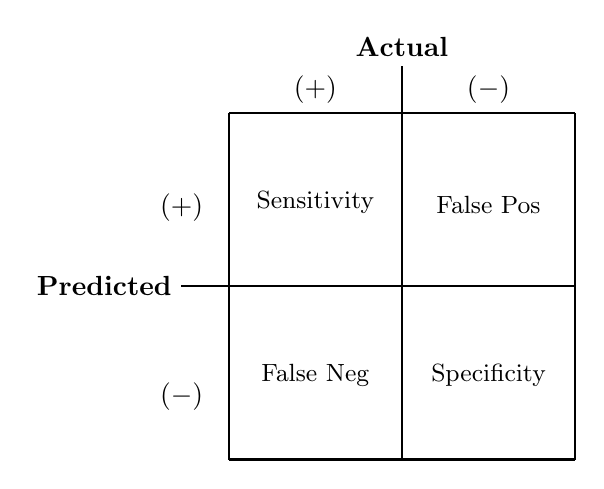
\begin{tikzpicture}[scale=2] %font=\scriptsize
    % Draw Basic Box
    \draw[thick] (0,0) -- (2.2,0);
    \draw[thick] (0,0) -- (0, 2.2);
    \draw[thick] (2.2,2.2) -- (2.2, 0);
    \draw[thick] (2.2,2.2) -- (0, 2.2);

    % Draw Box Ticks
    \draw[thick] (-0.3, 1.1) -- (2.2, 1.1);
    \draw[thick] (1.1, 0) -- (1.1, 2.5);

    % Box Labels
    % -- left side
    \coordinate[label=left:($+$)] (p1) at (-0.1,1.6);
    \coordinate[label=left:($-$)] (p2) at (-0.1,0.4);

    % -- top side
    \coordinate[label=above:($+$)] (p3) at (0.55, 2.2);
    \coordinate[label=above:($-$)] (p4) at (1.65, 2.2);

    % -- overall headers
    \coordinate[label=above:\textbf{Actual}] (p5) at (1.1, 2.5);
    \coordinate[label=left:\textbf{Predicted}] (p6) at (-0.3, 1.1);

    % Category Values
    \coordinate[label={\small{Sensitivity}}] (TP) at (0.55, 1.50);
    \coordinate[label={\small{False Pos}}] (FP) at (1.65, 1.50);
    \coordinate[label={\small{False Neg}}] (FN) at (0.55, 0.40);
    \coordinate[label={\small{Specificity}}] (TN) at (1.65, 0.40);
\end{tikzpicture}

\textbf{Receiver Operating Curve (ROC) / Area Under Curve (AUC)}

The ROC plots the true positive rate over the false positive rate at different classification thresholds. This generates a curve because when the threshold is 0, every prediction is positive, leading to a true positive rate of 1 and a false positive rate of 1. At the other extreme, when the threshold is set to 1, the false positive rate will be 0 and the true positive rate will also be 0.

A model which predicts randomly will produce an AUC value on an ROC plot of 0.5, and a perfect model which predicts correctly at every threshold would produce an AUC value of 1 (\cite{Aurélien2017} page 127). An AUC of 0 would be equivalent to 1 as the classification could be inverted.

\textbf{Conclusion}

The primary metric used to evaluate models in this project is the f1. Confusion matrices will also be used when providing further detail.

The selected metric must be applicable to both the iArsenic models and the machine learning based models. Because the iArsenic models do not provide a feature to change the classification threshold, a ROC cannot be produced. 

\section{Conclusion}

This chapter introduced existing prediction techniques used in related fields, including iArsenic which this project builds from, contextualised the application of these models with the black box problem, explored the possible tools available to implement and evaluate new models and explored which model types have been considered for development.

The following chapters include concepts detailed in this literature review, this chapter can be referred back to while reading further chapters.

The next chapter, Methodology, will outline exactly how these concepts have been researched and implemented throughout the development of this project. 